\chapter{Building Block View (Static View)}
\label{chapter{static_view}}

The following diagram shows the internal structure of RTA-SUM SOH:
\begin{figure}[H]
\centering
	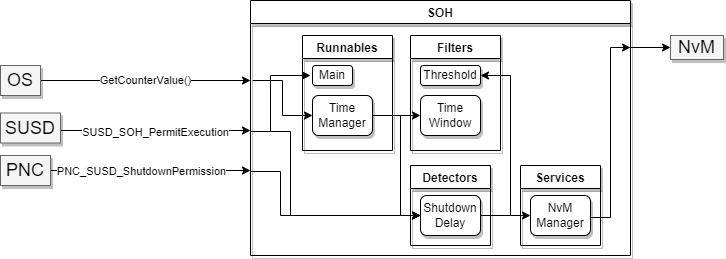
\includegraphics[width=\textwidth]{images/staticView.png}
	\caption{Generic Internal Module Structure}
	\label{fig:internal_components}
\end{figure}

The SUM\_SOH dependencies require that ECUs deploying the SUM\_SOH shall also deploy the following SUMs: SUM\_DIAG, SUM\_SUSD, SUM\_SSC, SUM\_PNC and SUM\_ERRH. By means of the RTE, it also interacts with the OS, BswM, DCM and WdgM (Figure~\ref{fig:internal_components}).


\section{Runnables}
The Runnables are functions that start when an event occurs.
They are the entry points of the feature implemented.
The Runnables present in the SOH are:
\begin{itemize}
	\item Main
	\item Init
	\item Time manager.
\end{itemize}

\section{Filters}
\label{section:filter}
The SUM\_SOH detectors can use one of two types of filtering:
\begin{itemize}
	\item Threshold filtering
	\item Time window filtering.
\end{itemize}
\subsection{Threshold Filter}

\subsection{Time Window Filter}
\label{subsection:timeWindowFilter}
\Requirement{008}
{
	The Time Window Filter requires:
	\begin{itemize}
		\item a 2-byte unsigned integer used as detection counter to maintain a raw count of the detected events
		\item a 3-byte unsigned integer used as time window
		\item a 2-byte unsigned integer used as DID counter to maintain a filtered count of the detected events.
	\end{itemize}	
}
{	\Satisfies{SRS_SOH 046} \Satisfies{SRS_SOH 051} \Satisfies{SRS_SOH 057}	}

\Requirement{009}
{
	Each detection counter requires:
	\begin{itemize}
		\item to be stored in a specific memory type according to Table \ref{table:detCounterMemType}
		\item a counter threshold calibration value associated with it.
	\end{itemize}
}
{	\Satisfies{SRS_SOH 047} \Satisfies{SRS_SOH 050}	\Satisfies{SRS_SOH 066} }

\Requirement{010}
{
	Each time window requires:
	\begin{itemize}
		\item to use seconds as its time base unit
		\item a time window threshold calibration value associated with it
		\item to reside in the same memory of the related detection counter.
	\end{itemize}
}
{	\Satisfies{SRS_SOH 052} \Satisfies{SRS_SOH 053}	\Satisfies{SRS_SOH 054}	}

\Requirement{011}
{
	Each DID counter requires to be stored in secure cumulative NVM.
}
{	\Satisfies{SRS_SOH 058}	}

\Requirement{012}
{
		\begin{longtable}{|l|l|}
\hline
\begin{minipage}{0.47\linewidth}\raggedright\vspace{.75ex}\textbf{Detection Counter Name}\vspace{.75ex}\end{minipage} & \begin{minipage}{0.47\linewidth}\raggedright\vspace{.75ex}\textbf{Memory Type}\vspace{.75ex}\end{minipage}\\
\hline\hline
\endfirsthead
\hline
\begin{minipage}{0.47\linewidth}\raggedright\vspace{.75ex}\textbf{Detection Counter Name}\vspace{.75ex}\end{minipage} & \begin{minipage}{0.47\linewidth}\raggedright\vspace{.75ex}\textbf{Memory Type}\vspace{.75ex}\end{minipage}\\
\hline\hline
\endhead
\hline
\endfoot
\hline
\endlastfoot
\begin{minipage}{0.47\linewidth}\raggedright\vspace{.75ex}SUM\_SOH\_ImmeReset\_Cntr\vspace{.75ex}\end{minipage} & \begin{minipage}{0.47\linewidth}\raggedright\vspace{.75ex}NonClearedRAM\vspace{.75ex}\end{minipage}\\\hline
\begin{minipage}{0.47\linewidth}\raggedright\vspace{.75ex}SUM\_SOH\_DelayedReset\_Cntr\vspace{.75ex}\end{minipage} & \begin{minipage}{0.47\linewidth}\raggedright\vspace{.75ex}NonClearedRAM\vspace{.75ex}\end{minipage}\\\hline
\begin{minipage}{0.47\linewidth}\raggedright\vspace{.75ex}SUM\_SOH\_DiagReset\_Cntr\vspace{.75ex}\end{minipage} & \begin{minipage}{0.47\linewidth}\raggedright\vspace{.75ex}AdaptableNVM\vspace{.75ex}\end{minipage}\\\hline
\begin{minipage}{0.47\linewidth}\raggedright\vspace{.75ex}SUM\_SOH\_StatNVM\_Cntr\vspace{.75ex}\end{minipage} & \begin{minipage}{0.47\linewidth}\raggedright\vspace{.75ex}RAM\vspace{.75ex}\end{minipage}\\\hline
\begin{minipage}{0.47\linewidth}\raggedright\vspace{.75ex}SUM\_SOH\_ActNVM\_Cntr\vspace{.75ex}\end{minipage} & \begin{minipage}{0.47\linewidth}\raggedright\vspace{.75ex}RAM\vspace{.75ex}\end{minipage}\\\hline
\begin{minipage}{0.47\linewidth}\raggedright\vspace{.75ex}SUM\_SOH\_PrivNVM\_Cntr\vspace{.75ex}\end{minipage} & \begin{minipage}{0.47\linewidth}\raggedright\vspace{.75ex}RAM\vspace{.75ex}\end{minipage}\\\hline
\begin{minipage}{0.47\linewidth}\raggedright\vspace{.75ex}SUM\_SOH\_ExcepOS\_Cntr\vspace{.75ex}\end{minipage} & \begin{minipage}{0.47\linewidth}\raggedright\vspace{.75ex}NonClearedRAM\vspace{.75ex}\end{minipage}\\\hline
\begin{minipage}{0.47\linewidth}\raggedright\vspace{.75ex}SUM\_SOH\_ServOS\_Cntr\vspace{.75ex}\end{minipage} & \begin{minipage}{0.47\linewidth}\raggedright\vspace{.75ex}NonClearedRAM\vspace{.75ex}\end{minipage}\\\hline
\begin{minipage}{0.47\linewidth}\raggedright\vspace{.75ex}SUM\_SOH\_StackOS\_Cntr\vspace{.75ex}\end{minipage} & \begin{minipage}{0.47\linewidth}\raggedright\vspace{.75ex}NonClearedRAM\vspace{.75ex}\end{minipage}\\\hline
\begin{minipage}{0.47\linewidth}\raggedright\vspace{.75ex}SUM\_SOH\_MemProtOS\_Cntr\vspace{.75ex}\end{minipage} & \begin{minipage}{0.47\linewidth}\raggedright\vspace{.75ex}NonClearedRAM\vspace{.75ex}\end{minipage}\\\hline
\begin{minipage}{0.47\linewidth}\raggedright\vspace{.75ex}SUM\_SOH\_TimeProtOS\_Cntr\vspace{.75ex}\end{minipage} & \begin{minipage}{0.47\linewidth}\raggedright\vspace{.75ex}NonClearedRAM\vspace{.75ex}\end{minipage}\\\hline
\begin{minipage}{0.47\linewidth}\raggedright\vspace{.75ex}SUM\_SOH\_ErrOS\_Cntr\vspace{.75ex}\end{minipage} & \begin{minipage}{0.47\linewidth}\raggedright\vspace{.75ex}NonClearedRAM\vspace{.75ex}\end{minipage}\\\hline
\begin{minipage}{0.47\linewidth}\raggedright\vspace{.75ex}SUM\_SOH\_ShutDown\_Cntr\vspace{.75ex}\end{minipage} & \begin{minipage}{0.47\linewidth}\raggedright\vspace{.75ex}AdaptableNVM\vspace{.75ex}\end{minipage}\\\hline
\begin{minipage}{0.47\linewidth}\raggedright\vspace{.75ex}SUM\_SOH\_ClearDiagInfo\_Cntr\vspace{.75ex}\end{minipage} & \begin{minipage}{0.47\linewidth}\raggedright\vspace{.75ex}RAM\vspace{.75ex}\end{minipage}\\\hline
\begin{minipage}{0.47\linewidth}\raggedright\vspace{.75ex}SUM\_SOH\_Reject\_ClearDiag\_Cntr\vspace{.75ex}\end{minipage} & \begin{minipage}{0.47\linewidth}\raggedright\vspace{.75ex}RAM\vspace{.75ex}\end{minipage}\\\hline
\begin{minipage}{0.47\linewidth}\raggedright\vspace{.75ex}SUM\_SOH\_DiagSession\_Cntr\vspace{.75ex}\end{minipage} & \begin{minipage}{0.47\linewidth}\raggedright\vspace{.75ex}Secure Cumulative NVM\vspace{.75ex}\end{minipage}\\\hline
\begin{minipage}{0.47\linewidth}\raggedright\vspace{.75ex}SUM\_SOH\_Accept\_DiagSession\_Cntr\vspace{.75ex}\end{minipage} & \begin{minipage}{0.47\linewidth}\raggedright\vspace{.75ex}Secure Cumulative NVM\vspace{.75ex}\end{minipage}\\\hline
\begin{minipage}{0.47\linewidth}\raggedright\vspace{.75ex}SUM\_SOH\_SecurityAccess\_Cntr\vspace{.75ex}\end{minipage} & \begin{minipage}{0.47\linewidth}\raggedright\vspace{.75ex}Secure Cumulative NVM\vspace{.75ex}\end{minipage}\\\hline
\begin{minipage}{0.47\linewidth}\raggedright\vspace{.75ex}SUM\_SOH\_MACfail\_TenAct\_Cntr\vspace{.75ex}\end{minipage} & \begin{minipage}{0.47\linewidth}\raggedright\vspace{.75ex}RAM\vspace{.75ex}\end{minipage}\\\hline
\begin{minipage}{0.47\linewidth}\raggedright\vspace{.75ex}SUM\_SOH\_ReplayCount\_Cntr\vspace{.75ex}\end{minipage} & \begin{minipage}{0.47\linewidth}\raggedright\vspace{.75ex}RAM\vspace{.75ex}\end{minipage}\\\hline
\begin{minipage}{0.47\linewidth}\raggedright\vspace{.75ex}SUM\_SOH\_SecP\_Cntr\vspace{.75ex}\end{minipage} & \begin{minipage}{0.47\linewidth}\raggedright\vspace{.75ex}RAM\vspace{.75ex}\end{minipage}\\\hline
\begin{minipage}{0.47\linewidth}\raggedright\vspace{.75ex}SUM\_SOH\_LocalStatFail\_Cntr\vspace{.75ex}\end{minipage} & \begin{minipage}{0.47\linewidth}\raggedright\vspace{.75ex}NonClearedRAM\vspace{.75ex}\end{minipage}\\\hline
\begin{minipage}{0.47\linewidth}\raggedright\vspace{.75ex}SUM\_SOH\_WdgM\_DEMErr\_Cntr\vspace{.75ex}\end{minipage} & \begin{minipage}{0.47\linewidth}\raggedright\vspace{.75ex}NonClearedRAM\vspace{.75ex}\end{minipage}\\\hline
\begin{minipage}{0.47\linewidth}\raggedright\vspace{.75ex}ERRH\_SOHSupFail\_Cntr\vspace{.75ex}\end{minipage} & \begin{minipage}{0.47\linewidth}\raggedright\vspace{.75ex}NonClearedRAM\vspace{.75ex}\end{minipage}\\\hline
\begin{minipage}{0.47\linewidth}\raggedright\vspace{.75ex}SOH\_ERRHSupFail\_Cntr\vspace{.75ex}\end{minipage} & \begin{minipage}{0.47\linewidth}\raggedright\vspace{.75ex}NonClearedRAM\vspace{.75ex}\end{minipage}\\\hline
\caption{\label{table:detCounterMemType}Detection Counter Memory Type}
\end{longtable}
}
{	\Satisfies{SRS_SOH 066}	}


\section{Reliability monitors}
The SUM\_SOH supports the following reliability monitors:
\begin{itemize}
	\item Reset Reliability monitor.
	\item Memory Status Reliability Monitor.
	\item Communication Reliability Monitor.
	\item Watchdog Manager Reliability Monitor.
	\item Platform Reliability Monitor.
\end{itemize}

\subsection{Platform Reliability Monitor}
\Requirement{001}
{
    The scope of this monitor is to keep track of the following platform related event:
    \begin{itemize}
		\item Shutdown Delay
    \end{itemize}
}
{
	\Satisfies{SRS_SOH 116} 
}

\subsubsection{Shutdown Delay Detector}
\Requirement{020}
{
    A Shutdown Delay is defined as a shutdown that does not occur within the ECU calibration shutdown threshold time.
}
{
	\Satisfies{SRS_SOH 117} \Satisfies{SRS_SOH 118} 
}

\Requirement{002}
{
    To handle the \textit{Shutdown Delay}, a Threshold filter is used  with the following variables:
    \begin{itemize}
		\item Counter           :	SUM_SOH_ShutDown_Cntr
		\item Counter Threshold	:	SUM_SOH_ShutDown_Thresh
		\item DID               :	SUM_SOH_DID_ShutDown_Cntr.
    \end{itemize}
	These variables are stored in a specific memory type according to Subsection \ref{subsection:timeWindowFilter}.
}
{
	\Satisfies{SRS_SOH 119} \Satisfies{SRS_SOH 120} \Satisfies{SRS_SOH 121}
	\Satisfies{SRS_SOH 132}
}

\Requirement{003}
{
	The Shutdown Delay Detector uses also an unsigned 2-byte integer timer SUM_SOH_ShutDown_Timer, to monitor the time duration that the ECU is taking to shut down.
	SUM_SOH_ShutDown_Timer uses seconds as its unit of time and is stored in RAM.\\
	A flag declares if the timer SUM_SOH_ShutDown_Timer has started or not.
}
{
	\Satisfies{SRS_SOH 122} \Satisfies{SRS_SOH 124} \Satisfies{SRS_SOH 125}  
}

\Requirement{021}
{
	Moreover, a calibration value SUM_SOH_ShutDown_Timer_Thresh associated with SUM_SOH_ShutDown_Timer defines the ECU calibration shutdown threshold time.
}
{
	\Satisfies{SRS_SOH 126}
}

\Requirement{028}{
	The flow of inputs and outputs is managed thanks to the following ports:
	\begin{itemize}
		\item SUSD_SOH_PermitExecution
		\item PNC_SUSD_ShutdownPermission.
	\end{itemize}
}{ \Satisfies{SRS_SOH 228} \Satisfies{SRS_SOH 229} }


\section{DIDs}
\subsection{DID Counters}
\subsubsection{DID 0xF091: SUM_SOH Platform Reliability Monitor}

\Requirement{022}
{
	SUM_SOH makes use of DID 0xF091 to maintain the results of Platform Reliability events thanks to the following parameters:
	\begin{itemize}
		\item SUM_SOH_DID_ShutDown_Cntr : a 2-byte unsigned integer used to maintain a filtered count of the occurences of shutdown delays.
	\end{itemize}
}
{	\Satisfies{SRS_SOH 036}	}




\section{Port Interfaces}
\label{subsection:interfaces}

All ECU types shall support Client / Server port interfaces.
All ECU types shall support Sender / Receiver port interfaces.

\begin{longtable}{|l|l|l|l|l|}
\hline
\begin{minipage}{0.42\linewidth}\raggedright\vspace{.75ex}\textbf{Port Interface}\vspace{.75ex}\end{minipage} & \begin{minipage}{0.07\linewidth}\raggedright\vspace{.75ex}\textbf{Port Type}\vspace{.75ex}\end{minipage} & \begin{minipage}{0.10\linewidth}\raggedright\vspace{.75ex}\textbf{P-Port}\vspace{.75ex}\end{minipage} & \begin{minipage}{0.10\linewidth}\raggedright\vspace{.75ex}\textbf{R-Port}\vspace{.75ex}\end{minipage} & \begin{minipage}{0.17\linewidth}\raggedright\vspace{.75ex}\textbf{Description}\vspace{.75ex}\end{minipage}\\
\hline\hline
\endfirsthead
\hline
\begin{minipage}{0.42\linewidth}\raggedright\vspace{.75ex}\textbf{Port Interface}\vspace{.75ex}\end{minipage} & \begin{minipage}{0.07\linewidth}\raggedright\vspace{.75ex}\textbf{Port Type}\vspace{.75ex}\end{minipage} & \begin{minipage}{0.10\linewidth}\raggedright\vspace{.75ex}\textbf{P-Port}\vspace{.75ex}\end{minipage} & \begin{minipage}{0.10\linewidth}\raggedright\vspace{.75ex}\textbf{R-Port}\vspace{.75ex}\end{minipage} & \begin{minipage}{0.17\linewidth}\raggedright\vspace{.75ex}\textbf{Description}\vspace{.75ex}\end{minipage}\\
\hline\hline
\endhead
\hline
\endfoot
\hline
\endlastfoot
\begin{minipage}{0.42\linewidth}\raggedright\vspace{.75ex}ERRH\_E\_BswEvent\vspace{.75ex}\end{minipage} & \begin{minipage}{0.07\linewidth}\raggedright\vspace{.75ex}Sender / Receiver\vspace{.75ex}\end{minipage} & \begin{minipage}{0.10\linewidth}\raggedright\vspace{.75ex}SUM\_ERRH\vspace{.75ex}\end{minipage} & \begin{minipage}{0.10\linewidth}\raggedright\vspace{.75ex}SUM\_SOH\vspace{.75ex}\end{minipage} & \begin{minipage}{0.17\linewidth}\raggedright\vspace{.75ex}Reception of DEM events which are routed from SUM\_ERRH to the SUM\_SOH for processing.\vspace{.75ex}\end{minipage}\\\hline
\begin{minipage}{0.42\linewidth}\raggedright\vspace{.75ex}SUSD\_SOH\_PermitExecution\vspace{.75ex}\end{minipage} & \begin{minipage}{0.07\linewidth}\raggedright\vspace{.75ex}Sender / Receiver\vspace{.75ex}\end{minipage} & \begin{minipage}{0.10\linewidth}\raggedright\vspace{.75ex}SUM\_SUSD\vspace{.75ex}\end{minipage} & \begin{minipage}{0.10\linewidth}\raggedright\vspace{.75ex}SUM\_SOH\vspace{.75ex}\end{minipage} & \begin{minipage}{0.17\linewidth}\raggedright\vspace{.75ex}Permit Execution interface to indicate that operating conditions are correct for the SUM\_SOH to execute its functions.\vspace{.75ex}\end{minipage}\\\hline
\begin{minipage}{0.42\linewidth}\raggedright\vspace{.75ex}PNC\_SUSD\_ShutdownPermission\vspace{.75ex}\end{minipage} & \begin{minipage}{0.07\linewidth}\raggedright\vspace{.75ex}Sender / Receiver\vspace{.75ex}\end{minipage} & \begin{minipage}{0.10\linewidth}\raggedright\vspace{.75ex}SUM\_PNC\vspace{.75ex}\end{minipage} & \begin{minipage}{0.10\linewidth}\raggedright\vspace{.75ex}SUM\_SOH\vspace{.75ex}\end{minipage} & \begin{minipage}{0.17\linewidth}\raggedright\vspace{.75ex}Notification to the SUM\_SOH of any active or not active partial networks.\vspace{.75ex}\end{minipage}\\\hline
\begin{minipage}{0.42\linewidth}\raggedright\vspace{.75ex}SSC\_E\_SecureMessageMonitoringEvents\vspace{.75ex}\end{minipage} & \begin{minipage}{0.07\linewidth}\raggedright\vspace{.75ex}Sender / Receiver\vspace{.75ex}\end{minipage} & \begin{minipage}{0.10\linewidth}\raggedright\vspace{.75ex}SUM\_SSC\vspace{.75ex}\end{minipage} & \begin{minipage}{0.10\linewidth}\raggedright\vspace{.75ex}SUM\_SOH\vspace{.75ex}\end{minipage} & \begin{minipage}{0.17\linewidth}\raggedright\vspace{.75ex}Notification of MAC failures along with their types.\vspace{.75ex}\end{minipage}\\\hline
\begin{minipage}{0.42\linewidth}\raggedright\vspace{.75ex}DIAG\_ECUResetRequest\vspace{.75ex}\end{minipage} & \begin{minipage}{0.07\linewidth}\raggedright\vspace{.75ex}Sender / Receiver\vspace{.75ex}\end{minipage} & \begin{minipage}{0.10\linewidth}\raggedright\vspace{.75ex}SUM\_DIAG\vspace{.75ex}\end{minipage} & \begin{minipage}{0.10\linewidth}\raggedright\vspace{.75ex}SUM\_SOH\vspace{.75ex}\end{minipage} & \begin{minipage}{0.17\linewidth}\raggedright\vspace{.75ex}Notification of a service 0x11 tester-initiated request for ECU Reset (not programming).\vspace{.75ex}\end{minipage}\\\hline
\begin{minipage}{0.42\linewidth}\raggedright\vspace{.75ex}SUSD\_SOH\_ResetOccured\vspace{.75ex}\end{minipage} & \begin{minipage}{0.07\linewidth}\raggedright\vspace{.75ex}Sender / Receiver\vspace{.75ex}\end{minipage} & \begin{minipage}{0.10\linewidth}\raggedright\vspace{.75ex}SUM\_SUSD\vspace{.75ex}\end{minipage} & \begin{minipage}{0.10\linewidth}\raggedright\vspace{.75ex}SUM\_SOH\vspace{.75ex}\end{minipage} & \begin{minipage}{0.17\linewidth}\raggedright\vspace{.75ex}Notification to the SUM\_SOH that a reset occurred. The type of reset is also communicated to the SUM\_SOH. Type of resets may be delayed or immediate.\vspace{.75ex}\end{minipage}\\\hline
\begin{minipage}{0.42\linewidth}\raggedright\vspace{.75ex}SSFM\_ClearDiagReq\vspace{.75ex}\end{minipage} & \begin{minipage}{0.07\linewidth}\raggedright\vspace{.75ex}Sender / Receiver\vspace{.75ex}\end{minipage} & \begin{minipage}{0.10\linewidth}\raggedright\vspace{.75ex}SUM\_SSFM\vspace{.75ex}\end{minipage} & \begin{minipage}{0.10\linewidth}\raggedright\vspace{.75ex}SUM\_SOH\vspace{.75ex}\end{minipage} & \begin{minipage}{0.17\linewidth}\raggedright\vspace{.75ex}Notification to the SUM\_SOH that a service 0x04 or a service 0x14 request was accepted or rejected.\vspace{.75ex}\end{minipage}\\\hline
\begin{minipage}{0.42\linewidth}\raggedright\vspace{.75ex}DIAG\_SOH\_DiagSessionRequest\vspace{.75ex}\end{minipage} & \begin{minipage}{0.07\linewidth}\raggedright\vspace{.75ex}Sender / Receiver\vspace{.75ex}\end{minipage} & \begin{minipage}{0.10\linewidth}\raggedright\vspace{.75ex}SUM\_DIAG\vspace{.75ex}\end{minipage} & \begin{minipage}{0.10\linewidth}\raggedright\vspace{.75ex}SUM\_SOH\vspace{.75ex}\end{minipage} & \begin{minipage}{0.17\linewidth}\raggedright\vspace{.75ex}Notification to the SUM\_SOH that a reprogramming request took place (service 0x10 subfunction 0x02).\vspace{.75ex}\end{minipage}\\\hline
\begin{minipage}{0.42\linewidth}\raggedright\vspace{.75ex}SSC\_SOH\_SecurityAccessError\vspace{.75ex}\end{minipage} & \begin{minipage}{0.07\linewidth}\raggedright\vspace{.75ex}Sender / Receiver\vspace{.75ex}\end{minipage} & \begin{minipage}{0.10\linewidth}\raggedright\vspace{.75ex}SUM\_SSC\vspace{.75ex}\end{minipage} & \begin{minipage}{0.10\linewidth}\raggedright\vspace{.75ex}SUM\_SOH\vspace{.75ex}\end{minipage} & \begin{minipage}{0.17\linewidth}\raggedright\vspace{.75ex}Notification to the SUM\_SOH of the occurrences of service 0x27 failures.\vspace{.75ex}\end{minipage}\\\hline
\begin{minipage}{0.42\linewidth}\raggedright\vspace{.75ex}BatteryVoltage\_DisableNVMWrite\vspace{.75ex}\end{minipage} & \begin{minipage}{0.07\linewidth}\raggedright\vspace{.75ex}Sender / Receiver\vspace{.75ex}\end{minipage} & \begin{minipage}{0.10\linewidth}\raggedright\vspace{.75ex}SUM\_SUSD\vspace{.75ex}\end{minipage} & \begin{minipage}{0.10\linewidth}\raggedright\vspace{.75ex}SUM\_SOH\vspace{.75ex}\end{minipage} & \begin{minipage}{0.17\linewidth}\raggedright\vspace{.75ex}Notification to the SUM\_SOH from SUM\_SUSD that vehicle battery voltage is too low to perform NVM writes.\vspace{.75ex}\end{minipage}\\\hline
\begin{minipage}{0.42\linewidth}\raggedright\vspace{.75ex}DIAG\_GetMEC\vspace{.75ex}\end{minipage} & \begin{minipage}{0.07\linewidth}\raggedright\vspace{.75ex}Sender / Receiver\vspace{.75ex}\end{minipage} & \begin{minipage}{0.10\linewidth}\raggedright\vspace{.75ex}SUM\_DIAG\vspace{.75ex}\end{minipage} & \begin{minipage}{0.10\linewidth}\raggedright\vspace{.75ex}SUM\_SOH\vspace{.75ex}\end{minipage} & \begin{minipage}{0.17\linewidth}\raggedright\vspace{.75ex}This interface is used by the SUM\_DIAG to communicate to SUM\_SOH to value of the MEC.\vspace{.75ex}\end{minipage}\\\hline
\begin{minipage}{0.42\linewidth}\raggedright\vspace{.75ex}DataServices<SOH>Data<n>\vspace{.75ex}\end{minipage} & \begin{minipage}{0.07\linewidth}\raggedright\vspace{.75ex}Client / Server\vspace{.75ex}\end{minipage} & \begin{minipage}{0.10\linewidth}\raggedright\vspace{.75ex}DCM\vspace{.75ex}\end{minipage} & \begin{minipage}{0.10\linewidth}\raggedright\vspace{.75ex}SUM\_SOH\vspace{.75ex}\end{minipage} & \begin{minipage}{0.17\linewidth}\raggedright\vspace{.75ex}To support the collection of Diagnostic DIDs that are part of the SUM\_SOH functionalities.\vspace{.75ex}\end{minipage}\\\hline
\begin{minipage}{0.42\linewidth}\raggedright\vspace{.75ex}DiagnosticReprogrammingRequest\vspace{.75ex}\end{minipage} & \begin{minipage}{0.07\linewidth}\raggedright\vspace{.75ex}Sender / Receiver\vspace{.75ex}\end{minipage} & \begin{minipage}{0.10\linewidth}\raggedright\vspace{.75ex}BswM\vspace{.75ex}\end{minipage} & \begin{minipage}{0.10\linewidth}\raggedright\vspace{.75ex}SUM\_SOH\vspace{.75ex}\end{minipage} & \begin{minipage}{0.17\linewidth}\raggedright\vspace{.75ex}Notification of a request to shutdown to reset as part of programming to jump to boot.\vspace{.75ex}\end{minipage}\\\hline
\begin{minipage}{0.42\linewidth}\raggedright\vspace{.75ex}SOH\_WdgM\_IndividualMode<1...n>\vspace{.75ex}\end{minipage} & \begin{minipage}{0.07\linewidth}\raggedright\vspace{.75ex}Mode Switch\vspace{.75ex}\end{minipage} & \begin{minipage}{0.10\linewidth}\raggedright\vspace{.75ex}WdgM\vspace{.75ex}\end{minipage} & \begin{minipage}{0.10\linewidth}\raggedright\vspace{.75ex}SUM\_SOH\vspace{.75ex}\end{minipage} & \begin{minipage}{0.17\linewidth}\raggedright\vspace{.75ex}Notification of WdgM local supervision failures occurrence for all supervised entities excluding the SUM\_SOH and the SUM\_ERRH.\newline \footnotesize{These interfaces replace the SOH\_BswM\_WdgM \_IndividualMode<1...n> interfaces described in GB8002.}\vspace{.75ex}\end{minipage}\\\hline
\begin{minipage}{0.42\linewidth}\raggedright\vspace{.75ex}SOH\_WdgM\_IndividualMode\_Errh\vspace{.75ex}\end{minipage} & \begin{minipage}{0.07\linewidth}\raggedright\vspace{.75ex}Mode Switch\vspace{.75ex}\end{minipage} & \begin{minipage}{0.10\linewidth}\raggedright\vspace{.75ex}WdgM\vspace{.75ex}\end{minipage} & \begin{minipage}{0.10\linewidth}\raggedright\vspace{.75ex}SUM\_SOH\vspace{.75ex}\end{minipage} & \begin{minipage}{0.17\linewidth}\raggedright\vspace{.75ex}Notification of the WdgM SUM\_ERRH local supervision failures occurrences. \newline \footnotesize{This interface replaces the SOH\_BsWM\_WdgM \_ERRHMode interface described in GB8002.}\vspace{.75ex}\end{minipage}\\\hline
\begin{minipage}{0.42\linewidth}\raggedright\vspace{.75ex}RP\_ErrorStatus\vspace{.75ex}\end{minipage} & \begin{minipage}{0.07\linewidth}\raggedright\vspace{.75ex}Mode Switch\vspace{.75ex}\end{minipage} & \begin{minipage}{0.10\linewidth}\raggedright\vspace{.75ex}BswM\vspace{.75ex}\end{minipage} & \begin{minipage}{0.10\linewidth}\raggedright\vspace{.75ex}SOH\vspace{.75ex}\end{minipage} & \begin{minipage}{0.17\linewidth}\raggedright\vspace{.75ex}This interface is used by the BswM to notify SUM\_SOH of SecP errors occurrences.\vspace{.75ex}\end{minipage}\\\hline
\begin{minipage}{0.42\linewidth}\raggedright\vspace{.75ex}NvMService\vspace{.75ex}\end{minipage} & \begin{minipage}{0.07\linewidth}\raggedright\vspace{.75ex}Client / Server\vspace{.75ex}\end{minipage} & \begin{minipage}{0.10\linewidth}\raggedright\vspace{.75ex}NvM\vspace{.75ex}\end{minipage} & \begin{minipage}{0.10\linewidth}\raggedright\vspace{.75ex}SOH\vspace{.75ex}\end{minipage} & \begin{minipage}{0.17\linewidth}\raggedright\vspace{.75ex}The interface provides services for the management and maintenance of NV data related to SOH Metrics.\vspace{.75ex}\end{minipage}\\\hline
\begin{minipage}{0.42\linewidth}\raggedright\vspace{.75ex}TCS\_SWC\_Clock\vspace{.75ex}\end{minipage} & \begin{minipage}{0.07\linewidth}\raggedright\vspace{.75ex}Client / Server\vspace{.75ex}\end{minipage} & \begin{minipage}{0.10\linewidth}\raggedright\vspace{.75ex}TCS\vspace{.75ex}\end{minipage} & \begin{minipage}{0.10\linewidth}\raggedright\vspace{.75ex}SOH\vspace{.75ex}\end{minipage} & \begin{minipage}{0.17\linewidth}\raggedright\vspace{.75ex}Provides Global Time for timestamp (unit 100ms).\vspace{.75ex}\end{minipage}\\\hline
\begin{minipage}{0.42\linewidth}\raggedright\vspace{.75ex}RoutineServices\_Clear\_SUM\_SOH\_logs\vspace{.75ex}\end{minipage} & \begin{minipage}{0.07\linewidth}\raggedright\vspace{.75ex}Client / Server\vspace{.75ex}\end{minipage} & \begin{minipage}{0.10\linewidth}\raggedright\vspace{.75ex}DCM\vspace{.75ex}\end{minipage} & \begin{minipage}{0.10\linewidth}\raggedright\vspace{.75ex}SOH\vspace{.75ex}\end{minipage} & \begin{minipage}{0.17\linewidth}\raggedright\vspace{.75ex}The interface provides services for the clear of the SOH Metrics.\vspace{.75ex}\end{minipage}\\\hline
\begin{minipage}{0.42\linewidth}\raggedright\vspace{.75ex}WdgM\_LocalSupervision\vspace{.75ex}\end{minipage} & \begin{minipage}{0.07\linewidth}\raggedright\vspace{.75ex} Client / Server\vspace{.75ex}\end{minipage} & \begin{minipage}{0.10\linewidth}\raggedright\vspace{.75ex}WdgM\vspace{.75ex}\end{minipage} & \begin{minipage}{0.10\linewidth}\raggedright\vspace{.75ex}SUM\_SOH\vspace{.75ex}\end{minipage} & \begin{minipage}{0.17\linewidth}\raggedright\vspace{.75ex}Notify the checkpoint reachement for implementing the Local Supervision.\vspace{.75ex}\end{minipage}\\\hline
\begin{minipage}{0.42\linewidth}\raggedright\vspace{.75ex}SOH\_ERRH\_ClearRID0x02C0\vspace{.75ex}\end{minipage} & \begin{minipage}{0.07\linewidth}\raggedright\vspace{.75ex}Client / Server\vspace{.75ex}\end{minipage} & \begin{minipage}{0.10\linewidth}\raggedright\vspace{.75ex}SUM\_ERRH\vspace{.75ex}\end{minipage} & \begin{minipage}{0.10\linewidth}\raggedright\vspace{.75ex}SUM\_SOH\vspace{.75ex}\end{minipage} & \begin{minipage}{0.17\linewidth}\raggedright\vspace{.75ex}The interface provides service for starting clear, all the metrics related to SUM\_SOH Local Supervision Detector implemented at ERRH side.\vspace{.75ex}\end{minipage}\\\hline
\begin{minipage}{0.42\linewidth}\raggedright\vspace{.75ex}SOH\_SUSD\_ShutdownPermission\vspace{.75ex}\end{minipage} & \begin{minipage}{0.07\linewidth}\raggedright\vspace{.75ex}Sender / Receiver\vspace{.75ex}\end{minipage} & \begin{minipage}{0.10\linewidth}\raggedright\vspace{.75ex}SUM\_SOH\vspace{.75ex}\end{minipage} & \begin{minipage}{0.10\linewidth}\raggedright\vspace{.75ex}SUM\_SUSD\vspace{.75ex}\end{minipage} & \begin{minipage}{0.17\linewidth}\raggedright\vspace{.75ex}Shutdown Permission interface to indicate that operating conditions are correct for the SUM\_SOH to execute the shutdown.\vspace{.75ex}\end{minipage}\\\hline
\end{longtable}




\section{Configuration}
\label{subsection:configuration}

SUM\_SOH is a SWC within the context of AUTOSAR.
It consists of static files and generated files.
SUM\_SOH configuration is done the same way as for standard BSW modules.
A parameter definition file is included with the module which allows users to configure the available parameters.
The generated files change based on the configuration.

For default values of calibration thresholds SOH is referring to the SDV-8002.
Configuration parameters shall be pre-compile, in other words the ECU behavior modification requires
a reflash of the complete application software.


\subsection{Included Containers}
\begin{longtable}{|l|l|l|}
\hline
\begin{minipage}{0.25\linewidth}\raggedright\vspace{.75ex}\textbf{Name}\vspace{.75ex}\end{minipage} & \begin{minipage}{0.17\linewidth}\raggedright\vspace{.75ex}\textbf{Multiplicity}\vspace{.75ex}\end{minipage} & \begin{minipage}{0.50\linewidth}\raggedright\vspace{.75ex}\textbf{Scope / Dependency}\vspace{.75ex}\end{minipage}\\
\hline\hline
\endfirsthead
\hline
\begin{minipage}{0.25\linewidth}\raggedright\vspace{.75ex}\textbf{Name}\vspace{.75ex}\end{minipage} & \begin{minipage}{0.17\linewidth}\raggedright\vspace{.75ex}\textbf{Multiplicity}\vspace{.75ex}\end{minipage} & \begin{minipage}{0.50\linewidth}\raggedright\vspace{.75ex}\textbf{Scope / Dependency}\vspace{.75ex}\end{minipage}\\
\hline\hline
\endhead
\hline
\endfoot
\hline
\endlastfoot
\begin{minipage}{0.25\linewidth}\raggedright\vspace{.75ex}SOHGeneral\vspace{.75ex}\end{minipage} & \begin{minipage}{0.17\linewidth}\raggedright\vspace{.75ex}1..1\vspace{.75ex}\end{minipage} & \begin{minipage}{0.50\linewidth}\raggedright\vspace{.75ex}General configuration parameters of the SOH\vspace{.75ex}\end{minipage}\\\hline
\begin{minipage}{0.25\linewidth}\raggedright\vspace{.75ex}SUSDConfigSet\vspace{.75ex}\end{minipage} & \begin{minipage}{0.17\linewidth}\raggedright\vspace{.75ex}1..1\vspace{.75ex}\end{minipage} & \begin{minipage}{0.50\linewidth}\raggedright\vspace{.75ex}This container contains the configuration parameters and sub containers of the SOH module supporting multiple SWC configuration sets\vspace{.75ex}\end{minipage}\\\hline
\end{longtable}

\subsection{SOHGeneral}
\label{subsection:SOHGen}

{
	\ConfigurationParameter{SOH_PermitExecution_Mask}
	{Mask that can be OR'd with the value supplied by PermitExecution to set any "don't care" bits to '1'.}
	{1..1}
	{ECUC-INTEGER-PARAM-DEF}
	{0..255}
	{190}
}

{
	\ConfigurationParameter{SOH_RunnableSOHMainPeriod}
	{Time in sec, for the periodicity of the Runnable_SOH_Main.}
	{1..1}
	{ECUC-INTEGER-PARAM-DEF}
	{0.001..0.2}
	{0.1}
}

{
	\ConfigurationParameter{SohGenerateInitRunnable}
	{This parameter, when configured to TRUE, generates a periodic Runnable Entity that is useful for calling the SOH_Init() function just once.}
	{1..1}
	{ECUC-BOOLEAN-PARAM-DEF}
	{NA}
	{0}
}

{
	\ConfigurationParameter{SohInitFuncPeriodicity}
	{This parameter is used to specify the time in ms for the periodicity of the runnable Runnable_SOH_Init.}
	{0..1}
	{ECUC-FLOAT-PARAM-DEF}
	{1.0...5000.0}
	{1000.0}
}

{
	\ConfigurationParameter{SOH\_StatNvM\_SupportEnabled}
	{This parameter is used to enable the Nvm Status Failure/Integrity Error class and the relative detector.}
	{1..1}
	{ECUC-BOOLEAN-PARAM-DEF}
	{NA}
	{1}
}

{
	\ConfigurationParameter{SOH\_ActNvM\_SupportEnabled}
	{This parameter is used to enable the Nvm Action Failure Error class and the relative detector.}
	{1..1}
	{ECUC-BOOLEAN-PARAM-DEF}
	{NA}
	{1}
}

{
	\ConfigurationParameter{SOH\_PrivNvM\_SupportEnabled}
	{This parameter is used to enable the Nvm Privilege class and the relative detector.}
	{1..1}
	{ECUC-BOOLEAN-PARAM-DEF}
	{NA}
	{1}
}
{
    \ConfigurationParameter{SOH_ExcepOS_SupportEnabled}
    {This parameter is used to enable the OS Hardware Protection Action Failure Error class and the relative detector.}
    {1..1}
    {ECUC-BOOLEAN-PARAM-DEF}
    {NA}
    {true}
}


{
    \ConfigurationParameter{SOH_ServOS_SupportEnabled}
    {This parameter is used to enable the OS Service Protection / Trusted Function Action Failure Error class and the relative detector.}
    {1..1}
    {ECUC-BOOLEAN-PARAM-DEF}
    {NA}
    {true}
}

{
    \ConfigurationParameter{SOH_StackOS_SupportEnabled}
    {This parameter is used to enable the OS Stack Fault class and the relative detector.}
    {1..1}
    {ECUC-BOOLEAN-PARAM-DEF}
    {NA}
    {true}
}

{
    \ConfigurationParameter{SOH_MemProtOS_SupportEnabled}
    {This parameter is used to enable the OS Memory Protection Failure Error class and the relative detector.}
    {1..1}
    {ECUC-BOOLEAN-PARAM-DEF}
    {NA}
    {true}
}


{
    \ConfigurationParameter{SOH_TimeProtOS_SupportEnabled}
    {This parameter is used to enable the OS Time Protection Action Failure Error class and the relative detector.}
    {1..1}
    {ECUC-BOOLEAN-PARAM-DEF}
    {NA}
    {true}
}


{
    \ConfigurationParameter{SOH_ErrOS_SupportEnabled}
    {This parameter is used to enable the OS Other OS Errors Action Failure Error class and the relative detector.}
    {1..1}
    {ECUC-BOOLEAN-PARAM-DEF}
    {NA}
    {true}
}



{\ConfigurationParameter{SOH\_RID\_02C0\_SOH\_Clear\_Log\_Reference}
{Reference to DCM RID 0x02C0 SOH Clear Logs}
{1..1}
{ECUC-REFERENCE-DEF}
{NA}
{-}}


\subsection{SOHConfigSet}
\label{subsection:SOHConfigSet}

\subsubsection{SOH\_ResetReliabilityMonitor}
This container includes the configuration parameters needed for the Reset Reliability Monitor detectors.

\paragraph{SOH\_ImmediateReset}
{\ConfigurationParameter{SUM_SOH_ImmeReset_Thresh_Init}
{Initial value of SUM_SOH_ImmeReset_Thresh}
{1..1}
{-}
{-..-}
{1}}

{\ConfigurationParameter{SUM_SOH_ImmeReset_TW_Thresh_Init}
{Initial value of SUM_SOH_ImmeReset_TW_Thresh}
{1..1}
{-}
{-..-}
{3600}}

{\ConfigurationParameter{SOH\_NvMImmResetDID\_Reference}
{Reference to the NVM DID Block}
{1..1}
{ECUC-REFERENCE-DEF}
{NA}
{-}}

{\ConfigurationParameter{SOH\_DID\_F08F\_ImmResetData\_Reference}
{Reference to DCM ImmReset Data}
{1..1}
{ECUC-REFERENCE-DEF}
{NA}
{-}}

\paragraph{SOH\_DelayedReset}

{\ConfigurationParameter{SUM_SOH_DelayedReset_Thresh_Init}
{Initial value of SUM_SOH_DelayedReset_Thresh}
{1..1}
{-}
{-..-}
{1}}

{\ConfigurationParameter{SUM_SOH_DelayedReset_TW_Thresh_Init}
{Initial value of SUM_SOH_DelayedReset_TW_Thresh}
{1..1}
{-}
{-..-}
{3600}}

{\ConfigurationParameter{SOH\_NvMDelayedResetDID\_Reference}
{Reference to the NVM DID Block}
{1..1}
{ECUC-REFERENCE-DEF}
{NA}
{-}}

{\ConfigurationParameter{SOH\_DID\_F08F\_DelayedResetData\_Reference}
{Reference to DCM DelayedReset Data}
{1..1}
{ECUC-REFERENCE-DEF}
{NA}
{-}}


\paragraph{SOH\_DiagnosticReset}

{\ConfigurationParameter{SUM_SOH_DiagReset_Thresh_Init}
{Initial value SUM_SOH_DiagReset_Thresh}
{1..1}
{-}
{-..-}
{1}}

{\ConfigurationParameter{SOH\_NvMDiagResetCntr\_Reference}
{Reference to the NVM Counter Block}
{1..1}
{ECUC-REFERENCE-DEF}
{NA}
{-}}

{\ConfigurationParameter{SOH\_NvMDiagResetDID\_Reference}
{Reference to the NVM DID Block}
{1..1}
{ECUC-REFERENCE-DEF}
{NA}
{-}}

{\ConfigurationParameter{SOH\_DID\_F08F\_DiagResetData\_Reference}
{Reference to DCM DiagReset Data}
{1..1}
{ECUC-REFERENCE-DEF}
{NA}
{-}}

\subsubsection{SOH\_MemoryStatusReliabilityMonitor}
This container includes the configuration parameters needed for the Memory Status Monitor detectors.

\underline{SOH\_NVMErrorsDetector}\newline
This container includes the configuration containers needed for the NVM Error detectors.

\paragraph{SOH\_StatusNVM}

{\ConfigurationParameter{SUM_SOH_StatNVM_Thresh_Init}
{Initial value of SUM_SOH_StatNVM_Thresh}
{1..1}
{-}
{-..-}
{1}}

{\ConfigurationParameter{SUM_SOH_StatNVM_TW_Thresh_Init}
{Initial value of SUM_SOH_StatNVM_TW_Thresh}
{1..1}
{-}
{-..-}
{3600}}

{\ConfigurationParameter{SOH\_NvMStatNVMDID\_Reference}
{Reference to the NVM DID Block}
{1..1}
{ECUC-REFERENCE-DEF}
{NA}
{-}}

{\ConfigurationParameter{SOH\_DID\_F090\_StatusNVM\_Reference}
{Reference to DCM StatusNVM Data}
{1..1}
{ECUC-REFERENCE-DEF}
{NA}
{-}}

\paragraph{SOH\_ActNVM}
{\ConfigurationParameter{SUM_SOH_ActNVM_Thresh_Init}
{Initial value of SUM_SOH_ActNVM_Thresh}
{1..1}
{-}
{-..-}
{1}}

{\ConfigurationParameter{SUM_SOH_ActNVM_TW_Thresh_Init}
{Initial value of SUM_SOH_ActNVM_TW_Thresh}
{1..1}
{-}
{-..-}
{3600}}

{\ConfigurationParameter{SOH\_NvMActNVMDID\_Reference}
{Reference to the NVM DID Block}
{1..1}
{ECUC-REFERENCE-DEF}
{NA}
{-}}

{\ConfigurationParameter{SOH\_DID\_F090\_ActNVM\_Reference}
{Reference to DCM ActNVM Data}
{1..1}
{ECUC-REFERENCE-DEF}
{NA}
{-}}

\paragraph{SOH\_PrivNVM}
{\ConfigurationParameter{SUM_SOH_PrivNVM_Thresh_Init}
{Initial value of SUM_SOH_PrivNVM_Thresh}
{1..1}
{-}
{-..-}
{1}}

{\ConfigurationParameter{SUM_SOH_PrivNVM_TW_Thresh_Init}
{Initial value of SUM_SOH_PrivNVM_TW_Thresh}
{1..1}
{-}
{-..-}
{3600}}

{\ConfigurationParameter{SOH\_NvMPrivNVMDID\_Reference}
{Reference to the NVM DID Block}
{1..1}
{ECUC-REFERENCE-DEF}
{NA}
{-}}

{\ConfigurationParameter{SOH\_DID\_F090\_PrivNVM\_Reference}
{Reference to DCM PrivNVM Data}
{1..1}
{ECUC-REFERENCE-DEF}
{NA}
{-}}


\underline{SOH\_OSErrorsDetector}\newline
The following configuration parameters are used to set the initial threshold value for each OS error class detection counter and their related time windows.
\vspace*{0.1in}

\paragraph{SOH_ExcepOS}
{\ConfigurationParameter{SUM_SOH_ExcepOS_Thresh_Init}
{Initial value of SUM_SOH_ExcepOS_Thresh}
{1..1}
{-}
{-..-}
{1}}

{\ConfigurationParameter{SUM_SOH_ExcepOS_TW_Thresh_Init}
{Initial value of SUM_SOH_ExcepOS_TW_Thresh}
{1..1}
{-}
{-..-}
{3600}}

{\ConfigurationParameter{SOH\_NvMExcepOSDID\_Reference}
{Reference to the NVM DID Block}
{1..1}
{ECUC-REFERENCE-DEF}
{NA}
{-}}

{\ConfigurationParameter{SOH\_DID\_F090\_ExcepOS\_Reference}
{Reference to DCM ExcepOS Data}
{1..1}
{ECUC-REFERENCE-DEF}
{NA}
{-}}


\paragraph{SOH_ServOS}
{\ConfigurationParameter{SUM_SOH_ServOS_Thresh_Init}
{Initial value of SUM_SOH_ServOS_Thresh}
{1..1}
{-}
{-..-}
{1}}

{\ConfigurationParameter{SUM_SOH_ServOS_TW_Thresh_Init}
{Initial value of SUM_SOH_ServOS_TW_Thresh}
{1..1}
{-}
{-..-}
{3600}}

{\ConfigurationParameter{SOH\_NvMServOSDID\_Reference}
{Reference to the NVM DID Block}
{1..1}
{ECUC-REFERENCE-DEF}
{NA}
{-}}

{\ConfigurationParameter{SOH\_DID\_F090\_ServOS\_Reference}
{Reference to DCM ServOS Data}
{1..1}
{ECUC-REFERENCE-DEF}
{NA}
{-}}

\paragraph{SOH_StackOS}
{\ConfigurationParameter{SUM_SOH_StackOS_Thresh_Init}
{Initial value of SUM_SOH_StackOS_Thresh}
{1..1}
{-}
{-..-}
{1}}

{\ConfigurationParameter{SUM_SOH_StackOS_TW_Thresh_Init}
{Initial value of SUM_SOH_StackOS_TW_Thresh}
{1..1}
{-}
{-..-}
{3600}}

{\ConfigurationParameter{SOH\_NvMStackOSDID\_Reference}
{Reference to the NVM DID Block}
{1..1}
{ECUC-REFERENCE-DEF}
{NA}
{-}}

{\ConfigurationParameter{SOH\_DID\_F090\_StackOS\_Reference}
{Reference to DCM StackOS Data}
{1..1}
{ECUC-REFERENCE-DEF}
{NA}
{-}}

\paragraph{SOH_MemProtOS}
{\ConfigurationParameter{SUM_SOH_MemProtOS_Thresh_Init}
{Initial value of SUM_SOH_MemProtOS_Thresh}
{1..1}
{-}
{-..-}
{1}}

{\ConfigurationParameter{SUM_SOH_MemProtOS_TW_Thresh_Init}
{Initial value of SUM_SOH_MemProtOS_TW_Thresh}
{1..1}
{-}
{-..-}
{3600}}

{\ConfigurationParameter{SOH\_NvMMemProtOSDID\_Reference}
{Reference to the NVM DID Block}
{1..1}
{ECUC-REFERENCE-DEF}
{NA}
{-}}

{\ConfigurationParameter{SOH\_DID\_F090\_MemProtOS\_Reference}
{Reference to DCM MemProtOS Data}
{1..1}
{ECUC-REFERENCE-DEF}
{NA}
{-}}

\paragraph{SOH_TimeProtOS}
{\ConfigurationParameter{SUM_SOH_TimeProtOS_Thresh_Init}
{Initial value of SUM_SOH_TimeProtOS_Thresh}
{1..1}
{-}
{-..-}
{1}}

{\ConfigurationParameter{SUM_SOH_TimeProtOS_TW_Thresh_Init}
{Initial value of SUM_SOH_TimeProtOS_TW_Thresh}
{1..1}
{-}
{-..-}
{3600}}

{\ConfigurationParameter{SOH\_NvMTimeProtOSDID\_Reference}
{Reference to the NVM DID Block}
{1..1}
{ECUC-REFERENCE-DEF}
{NA}
{-}}

{\ConfigurationParameter{SOH\_DID\_F090\_TimeProtOS\_Reference}
{Reference to DCM TimeProtOS Data}
{1..1}
{ECUC-REFERENCE-DEF}
{NA}
{-}}

\paragraph{SOH_ErrOS}
{\ConfigurationParameter{SUM_SOH_ErrOS_Thresh_Init}
{Initial value of SUM_SOH_ErrOS_Thresh}
{1..1}
{-}
{-..-}
{1}}

{\ConfigurationParameter{SUM_SOH_ErrOS_TW_Thresh_Init}
{Initial value of SUM_SOH_ErrOS_TW_Thresh}
{1..1}
{-}
{-..-}
{3600}}

{\ConfigurationParameter{SOH\_NvMErrOSDID\_Reference}
{Reference to the NVM DID Block}
{1..1}
{ECUC-REFERENCE-DEF}
{NA}
{-}}

{\ConfigurationParameter{SOH\_DID\_F090\_ErrOS\_Reference}
{Reference to DCM ErrOS Data}
{1..1}
{ECUC-REFERENCE-DEF}
{NA}
{-}}

{\ConfigurationParameter{SUM_SOH_ShutDown_Thresh_Init}
{Initial value of SUM_SOH_ShutDown_Thresh}
{1..1}
{-}
{-..-}
{1}}

{\ConfigurationParameter{SUM_SOH_ShutDown_Timer_Thresh_Init}
{Initial value of SUM_SOH_ShutDown_Timer_Thresh}
{1..1}
{-}
{-..-}
{60}}


\subsubsection{SOH_CommunicationReliabilityMonitor}
This container includes the configuration parameters needed for the Communication Reliability Monitor detectors. Here organized by events.

\paragraph{SOH_ClearDiagInfo}

{\ConfigurationParameter{SUM_SOH_ClearDiagInfo_Thresh_Init}
{Initial value of SUM_SOH_ClearDiagInfo_Thresh}
{1..1}
{-}
{-..-}
{1}}

{\ConfigurationParameter{SOH\_NvMClearDiagInfoDID\_Reference}
{Reference to the NVM DID Block}
{1..1}
{ECUC-REFERENCE-DEF}
{NA}
{-}}

{\ConfigurationParameter{SOH\_DID\_F092\_ClearDiagInfoDID\_Reference}
{Reference to DCM Clear Diag Infomation Data}
{1..1}
{ECUC-REFERENCE-DEF}
{NA}
{-}}

\paragraph{SOH_RejectClearDiag}

{\ConfigurationParameter{SUM_SOH_Reject_ClearDiag_Thresh_Init}
{Initial value of SUM_SOH_Reject_ClearDiag_Thresh}
{1..1}
{-}
{-..-}
{1}}

{\ConfigurationParameter{SOH\_NvMRejectClearDiagDID\_Reference}
{Reference to the NVM DID Block}
{1..1}
{ECUC-REFERENCE-DEF}
{NA}
{-}}

{\ConfigurationParameter{SOH\_DID\_F092\_RejectClearDiagDID\_Reference}
{Reference to DCM Reject Clear Diag Data}
{1..1}
{ECUC-REFERENCE-DEF}
{NA}
{-}}

\paragraph{SOH_DiagSession}

{\ConfigurationParameter{SUM_SOH_DiagSession_Thresh_Init}
{Initial value of SUM_SOH_DiagSession_Thresh}
{1..1}
{-}
{-..-}
{1}}

{\ConfigurationParameter{SOH\_NvMDiagSessionCntr\_Reference}
{Reference to the NVM DID Block}
{1..1}
{ECUC-REFERENCE-DEF}
{NA}
{-}}

{\ConfigurationParameter{SOH\_NvMDiagSessionDID\_Reference}
{Reference to the NVM DID Block}
{1..1}
{ECUC-REFERENCE-DEF}
{NA}
{-}}

{\ConfigurationParameter{SOH\_DID\_F092\_DiagSessionDID\_Reference}
{Reference to DCM Diag Session Data}
{1..1}
{ECUC-REFERENCE-DEF}
{NA}
{-}}

\paragraph{SOH_Accept_DiagSession}

{\ConfigurationParameter{SUM_SOH_Accept_DiagSession_Thresh_Init}
{Initial value of SUM_SOH_Accept_DiagSession_Thresh}
{1..1}
{-}
{-..-}
{1}}

{\ConfigurationParameter{SOH\_NvMAccept_DiagSessionCntr\_Reference}
{Reference to the NVM DID Block}
{1..1}
{ECUC-REFERENCE-DEF}
{NA}
{-}}

{\ConfigurationParameter{SOH\_NvMAccept_DiagSessionDID\_Reference}
{Reference to the NVM DID Block}
{1..1}
{ECUC-REFERENCE-DEF}
{NA}
{-}}

{\ConfigurationParameter{SOH\_DID\_F092\_Accept\_DiagSessionDID\_Reference}
{Reference to DCM Accept Diag Session Data}
{1..1}
{ECUC-REFERENCE-DEF}
{NA}
{-}}

\paragraph{SOH_SecurityAccess}

{\ConfigurationParameter{SUM_SOH_SecurityAccess_Thresh_Init}
{Initial value of SUM_SOH_SecurityAccess_Thresh}
{1..1}
{-}
{-..-}
{1}}

{\ConfigurationParameter{SOH\_NvMSecurityAccessCntr\_Reference}
{Reference to the NVM DID Block}
{1..1}
{ECUC-REFERENCE-DEF}
{NA}
{-}}

{\ConfigurationParameter{SOH\_NvMSecurityAccessDID\_Reference}
{Reference to the NVM DID Block}
{1..1}
{ECUC-REFERENCE-DEF}
{NA}
{-}}

{\ConfigurationParameter{SOH\_DID\_F092\_SecurityAccessDID\_Reference}
{Reference to DCM Security Access Data}
{1..1}
{ECUC-REFERENCE-DEF}
{NA}
{-}}

\paragraph{SOH_MACfailTenAct}

{\ConfigurationParameter{SUM_SOH_MACfail_TenAct_Thresh_Init}
{Initial value of SUM_SOH_MACfail_TenAct_Thresh}
{1..1}
{-}
{-..-}
{$2\times$ number of received MAC protected messages}}

{\ConfigurationParameter{SUM_SOH_MACfail_TenAct_TW_Thresh_Init}
{Initial value of SUM_SOH_MACfail_TenAct_TW_Thresh}
{1..1}
{-}
{-..-}
{2}}

{\ConfigurationParameter{SOH\_NvMMACfail_TenActDID\_Reference}
{Reference to the NVM DID Block}
{1..1}
{ECUC-REFERENCE-DEF}
{NA}
{-}}

{\ConfigurationParameter{SOH\_DID\_F092\_MACfail\_TenActDID\_Reference}
{Reference to DCM MAC fail type 1 and 2 Data}
{1..1}
{ECUC-REFERENCE-DEF}
{NA}
{-}}

\paragraph{SOH_ReplayCount}

{\ConfigurationParameter{SUM_SOH_ReplayCount_Thresh_Init}
{Initial value of SUM_SOH_ReplayCount_Thresh}
{1..1}
{-}
{-..-}
{1}}

{\ConfigurationParameter{SUM_SOH_ReplayCount_TW_Thresh_Init}
{Initial value of SUM_SOH_ReplayCount_TW_Thresh}
{1..1}
{-}
{-..-}
{3600}}

{\ConfigurationParameter{SUM_SOH_ReplayCount_Start_Thresh_Init}
{Initial value of SUM_SOH_ReplayCount_Start_Thresh}
{1..1}
{-}
{-..-}
{5}}

{\ConfigurationParameter{SOH\_NvMReplayCountDID\_Reference}
{Reference to the NVM DID Block}
{1..1}
{ECUC-REFERENCE-DEF}
{NA}
{-}}

{\ConfigurationParameter{SOH\_DID\_F092\_ReplayCountDID\_Reference}
{Reference to DCM MAC fail type 3 Data}
{1..1}
{ECUC-REFERENCE-DEF}
{NA}
{-}}

\paragraph{SOH_SecP}

{\ConfigurationParameter{SUM_SOH_SecP_Thresh_Init}
{Initial value of SUM_SOH_ReplayCount_Thresh}
{1..1}
{-}
{-..-}
{1}}

{\ConfigurationParameter{SUM_SOH_SecP_TW_Thresh_Init}
{Initial value of SUM_SOH_ReplayCount_TW_Thresh}
{1..1}
{-}
{-..-}
{3600}}

{\ConfigurationParameter{SOH\_NvMSecPDID\_Reference}
{Reference to the NVM DID Block}
{1..1}
{ECUC-REFERENCE-DEF}
{NA}
{-}}

{\ConfigurationParameter{SOH\_DID\_F092\_SecPDID\_Reference}
{Reference to DCM SecP Data}
{1..1}
{ECUC-REFERENCE-DEF}
{NA}
{-}}

\subsubsection{SOH\_WatchdogManagerReliabilityMonitor}
This container includes the configuration parameters needed for the Watchdog Manager Reliability Monitor detectors.


\paragraph{Local\_Supervision\_Failures\_Detector}
{\ConfigurationParameter{SUM\_SOH\_ImmeReset\_Thresh\_Init}
{Initial value of SUM_SOH_LocalStatFail_Thresh}
{1..1}
{-}
{-..-}
{1}}


{\ConfigurationParameter{SUM\_SOH\_LocalStatFail\_TW\_Thresh\_Init}
{Initial value of SUM_SOH_LocalStatFail_TW_Thresh}
{1..1}
{-}
{-..-}
{10}}

{\ConfigurationParameter{Supervised\_Entity\_Reference}
{Reference to a Supervised Entity container in the WdgM}
{0..Infinite}
{ECUC-REFERENCE-DEF}
{NA}
{-}}

{\ConfigurationParameter{SOH\_LocalSupervisionFailures\_DID\_counter\_Reference}
{Reference to the NVM Block related to SUM_SOH_DID_LocalStatFail_Cntr}
{1..1}
{ECUC-REFERENCE-DEF}
{NA}
{-}}

{\ConfigurationParameter{SOH\_DID\_F093\_LocalStatFail\_Reference}
{Reference to DCM LocalStatFail Data}
{1..1}
{ECUC-REFERENCE-DEF}
{NA}
{-}}

\paragraph{WdgM\_DEM\_Supervision\_Errors\_Detector}
{\ConfigurationParameter{SUM\_SOH\_WdgM\_DEMErr\_Thresh\_Init}
{Initial value of SUM_SOH_WdgM_DEMErr_Thresh}
{1..1}
{-}
{-..-}
{1}}


{\ConfigurationParameter{SUM\_SOH\_WdgM\_DEMErr\_TW\_Thresh\_Init}
{Initial value of SUM_SOH_WdgM_DEMErr_TW_Thresh}
{1..1}
{-}
{-..-}
{10}}


{\ConfigurationParameter{SOH\_WdgMDEMErr\_DID\_counter\_Reference}
{Reference to the NVM Block related to SUM_SOH_DID_WdgM_DEMErr_Cntr}
{1..1}
{ECUC-REFERENCE-DEF}
{NA}
{-}}

{\ConfigurationParameter{SOH\_DID\_F093\_WdgMDEMErr\_Reference}
{Reference to DCM WdgMDEMErr Data}
{1..1}
{ECUC-REFERENCE-DEF}
{NA}
{-}}

\paragraph{SUM\_ERRH\_Local\_Supervision\_Detector}
{\ConfigurationParameter{SOH_ERRHSupFail_Thresh_Init}
{Initial value of SOH_ERRHSupFail_Thresh}
{1..1}
{-}
{-..-}
{1}}


{\ConfigurationParameter{SOH\_ERRHSupFail\_TW\_Thresh\_Init}
{Initial value of SOH_ERRHSupFail_TW_Thresh}
{1..1}
{-}
{-..-}
{10}}


{\ConfigurationParameter{SOH\_ERRHLocalSupervisionFailures\_DID\_counter\_Reference}
{Reference to the NVM Block related to SUM_SOH_DID_ERRHSupFail_Cntr}
{1..1}
{ECUC-REFERENCE-DEF}
{NA}
{-}}

{\ConfigurationParameter{SOH\_DID\_F093\_ERRHSupFail\_Reference}
{Reference to DCM ERRHSupFail Data}
{1..1}
{ECUC-REFERENCE-DEF}
{NA}
{-}}

{\ConfigurationParameter{SOH\_DID\_F093\_ERRH\_Local\_Supervision\_Status\_Reference}
{Reference to DCM ERRH Local Supervision Status Data}
{1..1}
{ECUC-REFERENCE-DEF}
{NA}
{-}}

\subsubsection{SOH_PlatformReliabilityMonitor}
This container includes the configuration parameters needed for the Platform Reliability Monitor detectors. Here organized by events.

\paragraph{SOH_ShutDownDelay}

{\ConfigurationParameter{SUM_SOH_Shutdown_Thresh_Init}
{Initial value of SUM_SOH_Shutdown_Thresh}
{1..1}
{-}
{-..-}
{1}}

{\ConfigurationParameter{SUM_SOH_ShutDown_Timer_Thresh_Init}
{Initial value of SUM_SOH_ShutDown_Timer_Thresh}
{1..1}
{-}
{-..-}
{60}}

{\ConfigurationParameter{SOH\_NvMShutdownCntr\_Reference}
{Reference to the NVM DID Block}
{1..1}
{ECUC-REFERENCE-DEF}
{NA}
{-}}

{\ConfigurationParameter{SOH\_NvMShutdownDID\_Reference}
{Reference to the NVM DID Block}
{1..1}
{ECUC-REFERENCE-DEF}
{NA}
{-}}

{\ConfigurationParameter{SOH\_DID\_F091\_ShutdownDID\_Reference}
{Reference to DCM Shutdown DID counter Data}
{1..1}
{ECUC-REFERENCE-DEF}
{NA}
{-}}